\section{Dynamics in Asymmetric Circuits} \label{sec:stairs}

\subsection{Staircase Models}\emph{} \label{sub:stairs}

An interesting generalization of the random architecture is to consider ``staircases," which each consist of a series of gates, acting at cuts $x$, $x+1$, $x+2$, in sequential order. This would be a staircase moving to the right, but they can also move to the left. If there are $n$ gates in a staircase it is called an $n$-stair. They are called staircases because compared to figure~\ref{fig:tetris} they look like steps, as in figure~\ref{fig:stairs}. 
\begin{figure}
	\centering
	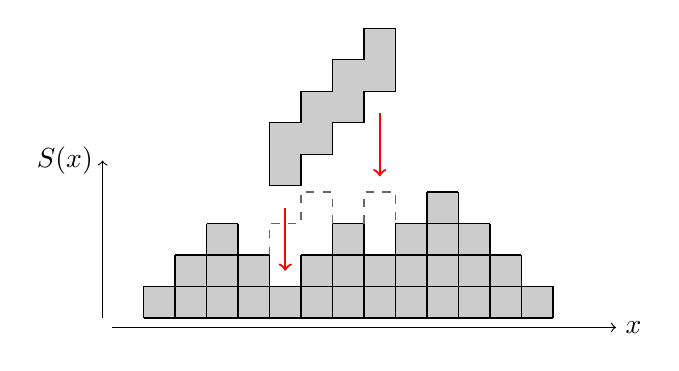
\begin{tikzpicture}[scale = .4]
\draw[->] (0, -.3) -- (16,-.3) node[right]{$x$};
\draw[->] (-.3,0) -- (-.3,5) node[left]{$S(x)$};
\fill[black!20] (1,0) -- (1,1) -- (2,1) -- (2,2) -- (3,2) -- (3,3) -- 
     			(4,3) -- (4,2) -- (5,2) -- (5,1) -- (6,1) -- (6,2) -- (7,2) -- (7,3) -- (8,3) -- (8,2) -- (9,2) -- (9,3) -- (10,3) -- (10,4) 
     			 -- (11,4) -- (11,3) -- (12,3) -- (12,2) -- (13,2) -- (13,1)  -- (14,1) -- (14,0);
     			 
\draw (1,0) -- (14,0);
\draw (1,1) -- (14,1);
\draw (2,2) -- (5,2);
\draw (6,2) -- (13,2);
\draw (3,3) -- (4,3);
\draw (7,3) -- (8,3);
\draw (9,3) -- (12,3);
\draw (10,4) -- (11,4);
\draw (1,0) -- (1,1);
\draw (2,0) -- (2,2);
\draw (3,0) -- (3,3);
\draw (4,0) -- (4,3);
\draw (5,0) -- (5,2);
\draw (6,0) -- (6,2);
\draw (7,0) -- (7,3);
\draw (8,0) -- (8,3);
\draw (9,0) -- (9,3);
\draw (10,0) -- (10,4);
\draw (11,0) -- (11,4);
\draw (12,0) -- (12,3);
\draw (13,0) -- (13,2);
\draw (14,0) -- (14,1);

\draw[fill=black!20] (5,5.2) -- (5,4.2) -- (6,4.2) -- (6,5.2) -- (7,5.2) --  
                     (7,6.2) --
					 (8,6.2) -- (8,7.2) -- (9,7.2) -- (9,8.2) -- (9,9.2) -- (8,9.2)
					 -- (8,8.2) -- (7,8.2) -- (7,7.2) -- (6,7.2) -- (6,6.2) -- (5,6.2)
					 -- (5,5.2);
\draw[thick, ->, red] (5.5,3.5) -- (5.5,1.5);
\draw[thick, ->, red] (8.5,6.5) -- (8.5,4.5);

\draw[dashed, black!60] (5,2) -- (5,3) -- (6,3) -- (6,4) -- (7,4) -- (7,3);
\draw[dashed, black!60] (8,3) -- (8,4) -- (9,4) -- (9,3);
\end{tikzpicture}
%\begin{tikzpicture}[scale = .3, cross/.style={path picture={ 
%		\draw[black]
%		(path picture bounding box.south east) -- (path picture bounding box.north west) (path picture bounding box.south west) -- (path picture bounding box.north east);
%}}]
%
%\draw[->] (0, -.3) -- (16,-.3) node[right]{$x$};
%\draw[->] (-.3,0) -- (-.3,5) node[left]{$S(x)$};
%\fill[black!20] (0,0) -- (3,3) -- (5,1) -- (7,3) -- (8,2) --
%(10,4) -- (14,0) ;
%\draw (0,0) -- (3,3);
%\draw (2,0) -- (4,2);
%\draw (4,0) -- (7,3);
%\draw (6,0) -- (10,4);
%\draw (8,0) -- (11,3);
%\draw (10,0) -- (12,2);
%\draw (12,0) -- (13,1);
%\draw (2,0) -- (1,1);
%\draw (4,0) -- (2,2);
%\draw (6,0) -- (3,3);
%\draw (8,0) -- (6,2);
%\draw (10,0) -- (7,3);
%\draw (12,0) -- (9,3);
%\draw (14,0) -- (10,4);
%\draw[dashed, black!60]  (5,3) -- (6,4);
%\draw[dashed, black!60]  (7,3) -- (6,4);
%\draw[dashed, black!60]  (6,2) -- (5,3);
%
%\draw[fill=black!20] (5,6) -- (6,5) -- (7,6) -- (6,7) -- (5,6);
%\draw[thick, ->, red] (6,4.5) -- (6,3);
%%\node [draw,circle,cross,minimum width=1](B) at (6,3.5){}; 
%\end{tikzpicture}

	\caption{\textbf{Staircase circuit architecture,} in which the gate at site $x$ is always followed by ones at sites $x+1, x+2$, making this a 3-stair. Note that not all gates are productive, only the ones that fall on sites that are local minima when they fall.}
	\label{fig:stairs}
\end{figure}
However, in the picture in which all sites are either up or down slopes, $n$-stair look like $n\times 1$ rectangles tilted $45^\circ$, as in figure~\ref{fig:diagstairs}.
\begin{figure}
	\centering
	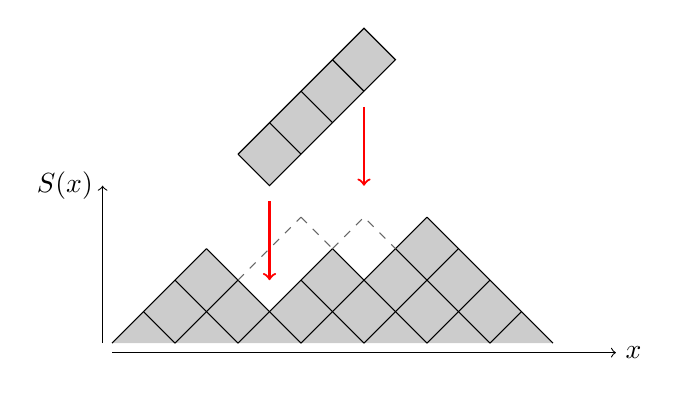
\begin{tikzpicture}[scale = .4]
\draw[->] (0, -.3) -- (16,-.3) node[right]{$x$};
\draw[->] (-.3,0) -- (-.3,5) node[left]{$S(x)$};
\fill[black!20] (0,0) -- (3,3) -- (5,1) -- (7,3) -- (8,2) --
				(10,4) -- (14,0) ;
\draw (0,0) -- (3,3);
\draw (2,0) -- (4,2);
\draw (4,0) -- (7,3);
\draw (6,0) -- (10,4);
\draw (8,0) -- (11,3);
\draw (10,0) -- (12,2);
\draw (12,0) -- (13,1);
\draw (2,0) -- (1,1);
\draw (4,0) -- (2,2);
\draw (6,0) -- (3,3);
\draw (8,0) -- (6,2);
\draw (10,0) -- (7,3);
\draw (12,0) -- (9,3);
\draw (14,0) -- (10,4);

\draw[fill=black!20] (4,6) -- (5,5) -- (6,6) -- (7,7) -- (8,8) -- (9,9) --
					 (8,10) -- (7,9) -- (6,8) -- (5,7) -- (4,6);
\draw (6,6) -- (5,7);
\draw (7,7) -- (6,8);
\draw (8,8) -- (7,9);
%\draw (9,9) -- ()
\draw[thick, ->, red] (5,4.5) -- (5,2);
\draw[thick, ->, red] (8,7.5) -- (8,5);

\draw[dashed, black!60] (4,2) -- (6,4);
\draw[dashed, black!60] (6,4) -- (7,3);
\draw[dashed, black!60] (7,3) -- (8,4) -- (9,3);
\end{tikzpicture}
%\begin{tikzpicture}[scale = .3, cross/.style={path picture={ 
%		\draw[black]
%		(path picture bounding box.south east) -- (path picture bounding box.north west) (path picture bounding box.south west) -- (path picture bounding box.north east);
%}}]
%
%\draw[->] (0, -.3) -- (16,-.3) node[right]{$x$};
%\draw[->] (-.3,0) -- (-.3,5) node[left]{$S(x)$};
%\fill[black!20] (0,0) -- (3,3) -- (5,1) -- (7,3) -- (8,2) --
%(10,4) -- (14,0) ;
%\draw (0,0) -- (3,3);
%\draw (2,0) -- (4,2);
%\draw (4,0) -- (7,3);
%\draw (6,0) -- (10,4);
%\draw (8,0) -- (11,3);
%\draw (10,0) -- (12,2);
%\draw (12,0) -- (13,1);
%\draw (2,0) -- (1,1);
%\draw (4,0) -- (2,2);
%\draw (6,0) -- (3,3);
%\draw (8,0) -- (6,2);
%\draw (10,0) -- (7,3);
%\draw (12,0) -- (9,3);
%\draw (14,0) -- (10,4);
%%\draw[dashed, black!60]  (5,3) -- (6,4);
%%\draw[dashed, black!60]  (7,3) -- (6,4);
%%\draw[dashed, black!60]  (6,2) -- (5,3);
%
%\draw[fill=black!20] (5,6) -- (6,5) -- (7,6) -- (6,7) -- (5,6);
%\draw[thick, ->, red] (6,4.5) -- (6,3);
%%\node [draw,circle,cross,minimum width=1](B) at (6,3.5){}; 
%\end{tikzpicture}

	\caption{\textbf{Another picture of the staircase architecture.} Note that this picture results in the same final state.}
	\label{fig:diagstairs}
\end{figure}

\subsection{Behavior Ignoring Correlations} \emph{}\label{sub:anal}

Under certain approximations the entanglement entropy behaves analytically. One important approximation (described in section \ref{subsub:determ}) is that the Hilbert space at each site is large enough that almost all gates will in general maximally entangle the two sites on which they act. Other simplifying assumptions include ignoring correlations in ups and downs and ignoring second- and higher-order derivatives in $S(x,t)$. Combining these two assumptions, we arrive at uncorrelated entropy environments, which may be described only by their slope, $m$.

\subsubsection{Small Stairs} \label{subsub:smallstairs} \emph{}

The smallest stairs are 1-stairs, which are just individual gates. For an entropy surface with constant slope $m$ and no correlations, each step from one site to the next has probability $\frac{1+m}{2}$ of being up and $\frac{1-m}{2}$ of being down. The assumption that there are no correlations is exact in the 1-stair case. Consider a gate operating on site $n$ at time $t$. For the gate to increase the entropy $S(n)$, it must be the case that $S(n)<S(n-1), S(n+1)$. The probability of this is $\frac{1+m}{2} \frac{1-m}{2} = \frac{1-m^2}{4}$. In this case we have $S(n,t+1)=S(n,t)+2$, because the gate increases the entropy to be great than that of its neighbors. Then if the gates arrive with a rate $\Gamma$, we have
\begin{align}
\pd{S}{t} = \Gamma\frac{1-m^2}{2}.
\end{align}
Useful checks of this formula are that the entropy does not increase at maximal or minimal slope $m=1,-1$, and that at $m=0$, $\pd{S}{t}=\Gamma/2$, half the brickwork value. The latter rate makes sense because in the case of the brickwork circuit all gates are guaranteed to raise the entropy, while here only half\footnote{Fix this} will have an effect.

2-stairs consist of one gate acting at site $n$ and one at site $n+1$. The entropy production of these gates is affected by the slope between them and the two slopes on either side. There are 8 possible configurations of those three slopes, but only 4 result in entropy growth, as shown in table~\ref{tab:2stair}. Although there will be correlation built up by the 2-stair architecture, we can still make the assumption that there are no correlations. The average growth rate is then approximately 
\begin{align}
\pd{S}{t} = \Gamma\frac{1-m^2}{2}\frac{5+m}{4},
\end{align}
where $\Gamma$ is the rate of gates, so the rate of 2-stairs is $2\Gamma$.

\begin{table}
	\centering
	\begin{tabular}{ccc}
		Initial and Final 
		Configuration        & Probability         & Productivity\\
		$d\,u\,d\to u\,d\,d$ & $\frac{1-m^2}{4}\frac{1-m}{2}$ & 2\\
		$d\,u\,u\to u\,u\,d$ & $\frac{1-m^2}{4}\frac{1+m}{2}$ & 4\\
		$d\,d\,u\to d\,u\,d$ & $\frac{1-m^2}{4}\frac{1-m}{2}$ & 2\\
		$u\,d\,u\to u\,u\,d$ & $\frac{1-m^2}{4}\frac{1+m}{2}$ & 2
	\end{tabular}
	\caption{The four configurations that result in entropy growth for 2-stairs, their relative proportions assuming an uncorrelated entropy distribution, and the growth in entropy generated by a 2-stair falling on that configuration. The four configurations that do not result in entropy growth are $u\,u\,u, d\,d\,d, u\,d\,d,$ and $u\,u\,d$.}
	\label{tab:2stair}
\end{table}

\subsubsection{Larger Stairs} \emph{} \label{subsub:largestairs}

We can determine the growth rate for arbitrary length stairs through a recursive relationship. Consider a staircase made of $n$ gates. Its growth rate will be proportional to the gate rate normalized by the number of gates per stair, so we can write
\begin{align}
\pd{S}{t} = \frac{\Gamma}{n}R_n(m), \label{eqn:growthrate}
\end{align}
where $R_n(m)$ is the average entropy production of an $n$-stair. To find an equation for $R_n(m)$, note that the first $n-1$ gates have the same entropy production as the $(n-1)$-stair. Then the $n$th gate will produce another 2 units of entropy if the last step is up, but not if all $n+1$ steps are up. This is captured by the recursive formula
\begin{align}
R_n(m) = R_{n-1}(m)+2\frac{1+m}{2} - 2\left(\frac{1+m}{2}\right)^{n+1}. \label{eqn:raterecur}
\end{align}
Figure~\ref{fig:growthrates} contains a graph of some growth rates $\th{n}R_n(m)$ as a function of $m$.

\begin{figure}
	\centering
	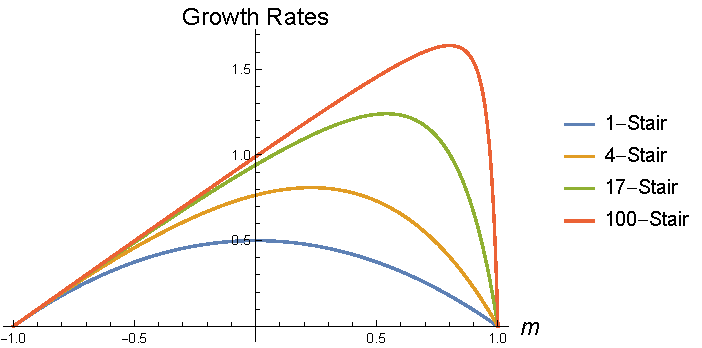
\includegraphics[width=.5\textwidth]{analrates.png}
	\caption{Growth rates for 1-, 4-, 17-, and 100-stairs as a function of slope $m$. As stair length increases, the growth rate asymptotes to the function $\pd{S}{t} = m+1$.}
	\label{fig:growthrates}
\end{figure}

Note that with increasing stair length the growth rate asymptotes to the function $\pd{S}{t} = m+1$. There are two ways to reach this behavior. The first, which matches the order of the current reasoning, is to start with infinite spatial support and take the stair length $n\to\infty$. Alternatively, start with a finite spin chain with length $N$ and periodic boundary conditions, and set the stair length to $N$. Now a single gate acts on site $1,2,3\dots N$, before wrapping around to act at site 1 again. 

The maximal growth rate occurs when the slope is near-maximal, with only a single down step. This corresponds to a slope of $\frac{N-2}{N}$. Then with only a single local minimum in the entropy function, the local minimum moves one site to the right with each gate. Every gate that acts raises the entropy, resulting in an entropy gain of 2 per gate. Of course for a slope of 1, there is still no entropy generation.

If there are 2 down steps, for a slope of $\frac{N-4}{N}$, the entropy generation is almost the same. One local minimum still moves to the right with the leading edge of the staircase. However, once per staircase (once every $N$ gates), one down step is next to the other down step. This results in no entropy growth for that step, for an average entropy gain of $2\frac{N-1}{N}$. Further discussion of the dynamics with near-maximal slope appear in section~\ref{subsub:nearmax}.

This pattern continues as the slope decreases. With $\l$ down steps, the slope is $\frac{N-2\l}{N}$ and the average growth rate is $2\frac{N-\l}{N} = m+1$. At $m = -1$ there is no growth, as expected. At $m=0$, the growth rate is 1, the same as in the brickwork model. With no slope, the steps alternate between up and down, so that half of the gates in any stair are effective, explaining the connection to the brickwork model.

\subsubsection{Near-Maximal Slopes} \emph{} \label{subsub:nearmax}

When the slope is near its largest possible value, so that the entropy increases at nearly every site, it is possible to isolate the behavior of the few down steps. Since gates can only act between a down step and an up step, these ``particles" follow a deterministic behavior and control the entropy growth in the circuit.

Consider a stair with its first gate acting between sites $i$ and $i+1$ and its last gate between $j$ and $j+1$. If there are no down steps in this region, the gate has no effect. 

\subsection{Ergodicity and Stability}\footnote{The following section describes an attempt to calculate steady state correlations. I haven't been successful in doing this yet, but I wanted to write it up in case it proves useful.} \label{sub:erg}\emph{}

A Markov process is one in which the future state depends only on the current state, not the past. Label the states $s_i$ and define $p_{i,t}$ as the probability that the system is in state $s_i$ at time $t$. When there is a constant probability $S_{ij}$ of transitioning from state $j$ to state $i$\footnote{Is this true of all Markov processes?} it is possible to write the transition matrix $S$ such that $p_{i,t+1}= S_{ij}p_{j,t}$. Since the product of the transition matrix and a probability vector gives the probabilities at the next time step, the transition matrix for $t$ time steps is just $S^t$. Under certain conditions\footnote{Figure these out.} the multi-step transition matrix approaches a constant matrix with all columns equal to the same vector $v^*$,
\begin{align}
\lim\limits_{t\to \infty}S^t = S^* = \begin{bmatrix}
\vdots & \vdots &  & \vdots\\
p^* & p^* & \cdots & p^*\\
\vdots & \vdots &  & \vdots\\
\end{bmatrix}.
\end{align}
Then the probability after a long time is the vector $p^*$ for any initial state.

The transition matrix can also be written as $S = 1+T$. The columns of $T$ must sum to 0 to preserve probabilities. From $S^*p^* = p^*,$ it must be true that $Tp^*=0$. This definition provides an easier route to finding $p^*$.

\subsubsection{Stable State in Random Architecture} \emph{} \label{subsub:randstate}

This analysis can be used to find the correlations present in the steady states of staircase architectures. Consider the 1-stair circuit, and enumerate 2-site (3-cut) states by the slope at the 2 sites: $s_1 = d\,d,\; s_2 = d\,u$, etc. Since at every time step there is an equal probability of a gate falling at any site, the transition matrix is the matrix product of single-cut transition matrices $P_{N} = \prod_NP_{1}\otimes$, where the single-cut transition matrix is 
\begin{align}
P_1 = \begin{bmatrix}
1-\frac{1+m}{2}\Gamma & 0      & \frac{1-m}{2}\Gamma & 0\\
\frac{1+m}{2}\Gamma & 1-\Gamma & 0                   & \frac{1-m}{2}\Gamma\\
0                   & \Gamma   & 1-\Gamma            & 0\\
0                   & 0        & \frac{1+m}{2}\Gamma & 1 - \frac{1-m}{2}\Gamma
\end{bmatrix}. \label{eqn:1sitetrans}
\end{align}
The $m$ dependence comes from the possibility of a gate acting on the left or right cut, which depends on the probability of the next slope being up or down.
The equilibrium state is
\begin{align}
v^* = \begin{pmatrix}
\frac{(1-m)^2}{4} \\ 
\frac{1+m}{2}\frac{1-m}{2} \\
\frac{1-m}{2}\frac{1+m}{2} \\
\frac{(1+m)^2}{4}
\end{pmatrix} = \begin{pmatrix}
\frac{1-m}{2} \\ \frac{1+m}{2}
\end{pmatrix} \otimes \begin{pmatrix}
\frac{1-m}{2} \\ \frac{1+m}{2}
\end{pmatrix},
\end{align}
which is uncorrelated, showing that the assumption of lack of correlation (used in equation~\ref{eqn:1sitetrans}) is consistent. Markov's theorem states that if all states are reachable from all other states\footnote{Probably introduce this earlier.} then the system is ergodic. An ergodic system contains only one equilibrium state, so the uncorrelated state is the unique equilibrium state.

\subsubsection{Stable States in Larger Staircases} \emph{} \label{subsub:stairstate}

Finding the stable state in the staircase models is more difficult. Since there are in fact correlations, a transition matrix built using the same method as in equation~\ref{eqn:1sitetrans} would be inexact. One possibility is to assume that the preceding and succeeding slopes are uncorrelated but to consider larger and larger subsystems (instead of the 2 slopes used previously).\footnote{I've made progress on this but haven't finished it.}

\subsection{Numerical Simulation} \emph{}\label{sub:num}

To simulate the entropy growth in infinite spin chains with non-zero slope, we use finite chains with periodic boundary conditions, where one end of the chain is attached to the other with an offset. The spin chains are initialized with a highly correlated\footnote{A next step is to fix the initialization so that the states start uncorrelated.} entropy function with the given slope. Since larger gates will generate different correlation, growth rates are calculated for only the latter part of the simulation, ensuring that the entropy is in its equilibrium state.

\subsubsection{Measuring Growth Rates} \emph{} \label{subsub:growthrates}

Growth rates for stairs of various lengths are shown in figure~\ref{fig:compareRates}. As length increases, the growth rate follows the same pattern as predicted, increasing with the maximum moving right. 
\begin{figure}
	\centering
	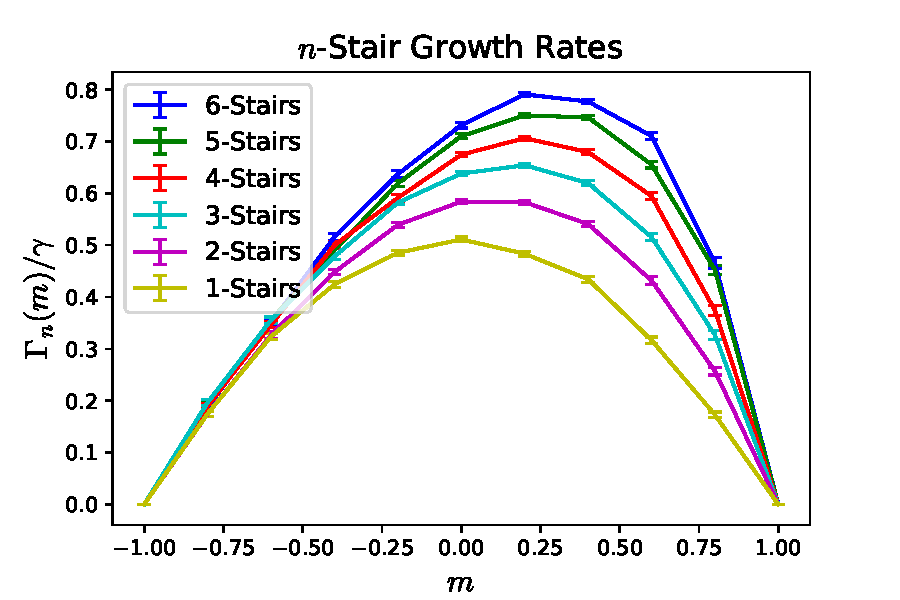
\includegraphics[width=.5\textwidth]{compareRates.pdf}
	\caption{\textbf{Growth rates for different length stairs.} All growth rates were calculated using a 100-site spin chain with offset periodic boundary conditions. Rates were calculated from the application of 100,000 gates, averaged over the last 80\% of the gates in order to build up correlations.}
	\label{fig:compareRates}
\end{figure}

For 1-stairs (the random architecture), the measured growth rate is slightly larger than predicted, seen in figure~\ref{fig:1stairRates}.
\begin{figure}
	\centering
	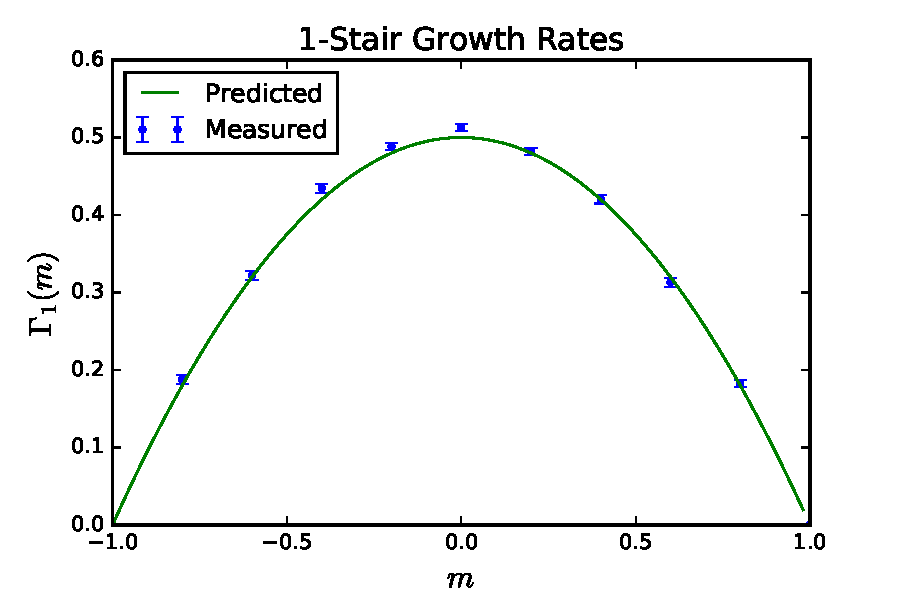
\includegraphics[width=.5\textwidth]{1stairRates.pdf}
	\caption{\textbf{Measured and analytic growth rates} for the 1-stair architecture. Note that the measured rate is slightly higher. Since the assumption of un-correlation is exact for 1-stairs, this difference is assumed to be due to second order derivatives in the slope and finite length effects.}
	\label{fig:1stairRates}
\end{figure}
There are two main differences between the analytic and measured setups. For the analytic result, the chain is infinite and the entropy function is assumed to be linear and uncorrelated. Since the assumption of un-correlation is exact for 1-stairs, this difference is assumed to be due to second order derivatives in the slope and finite length effects.

Stairs of length greater than 1 do however generate correlations. Figure~\ref{fig:6stairRates} shows the growth rates for 6-stairs. 
\begin{figure}
	\centering
	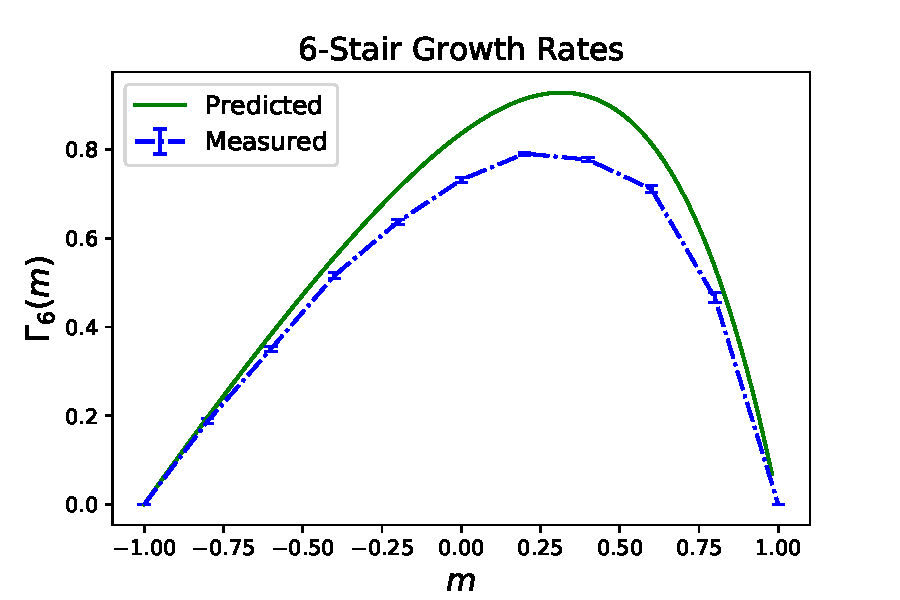
\includegraphics[width=.5\textwidth]{6stairRates.pdf}
	\caption{\textbf{Measured and predicted growth rates} for the 6-stair architecture. The measured rate is now lower than predicted, implying that the correlations built up by the stairs act to lower their entropy production.}
	\label{fig:6stairRates}
\end{figure}
The notable difference in growth rate here is probably due to correlations created by the 6-stairs. Hopefully reasoning similar to that in section~\ref{sub:erg} will be able to predict the correlation so that its effect, at least to first order, can be calculated. This would allow a much closer approximation than that in figure~\ref{fig:6stairRates}

\subsubsection{Measuring Correlations} \emph{} \label{subsub:correlations}

The first step in understanding the difference between predicted and measured behavior is understanding the correlations introduced by the gates. Figure~\ref{fig:stairCorrel} shows the initial and final correlations for the 1- and 3-stair circuits. Both curves were created by averaging over the correlation in the second half of a 10,000 step run, averaged over 10 runs.
\begin{figure}
	\centering
	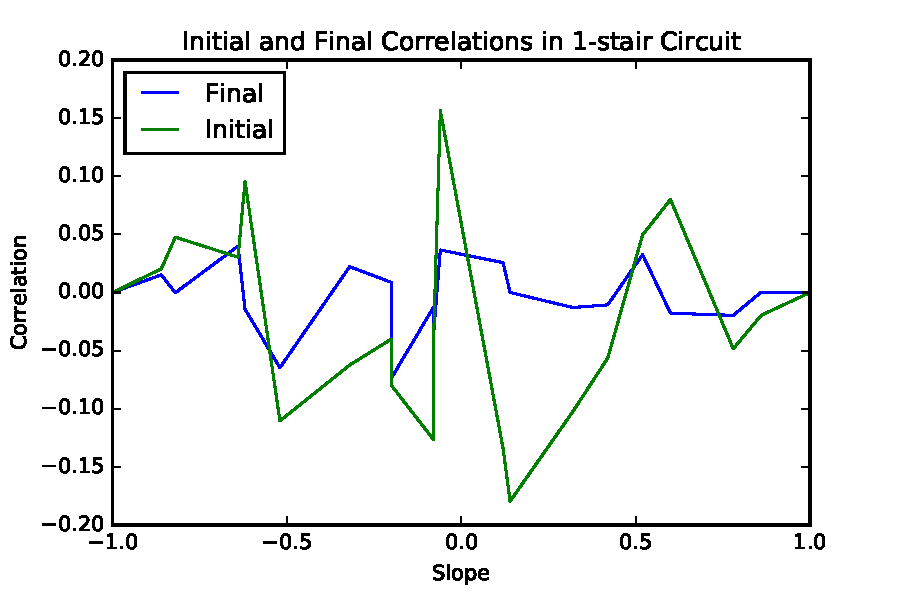
\includegraphics[width=.495\textwidth]{1stairCorrel}
	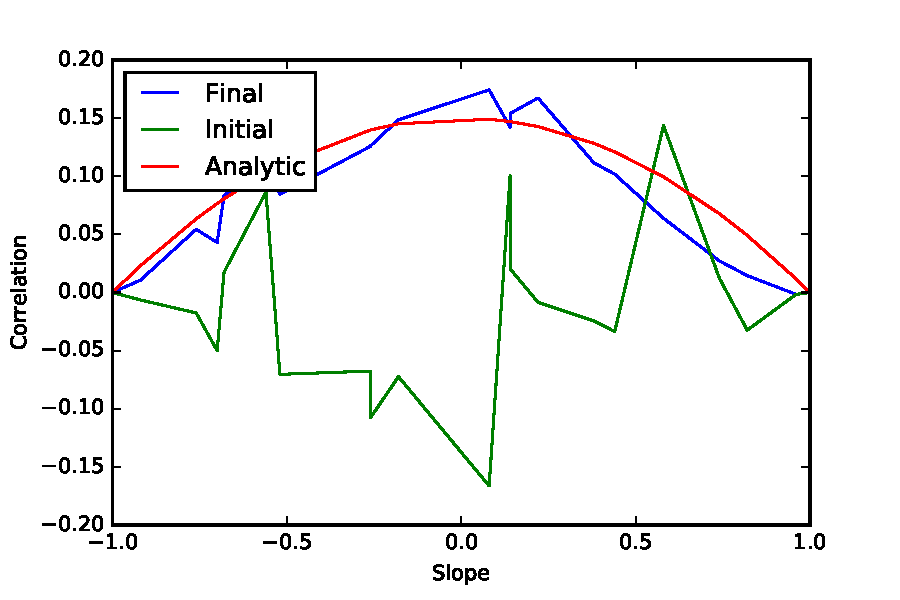
\includegraphics[width=.495\textwidth]{3stairCorrel}
	\caption{\textbf{Correlations created by 1- and 3-stair circuits.} The initial correlation curve shows that because of the initialization procedure the slope-0 state is perfectly anti-correlated. However, the correlation quickly equilibrates (see figure~\ref{fig:corrgrowth}). The 3-stair circuit reaches a more highly-correlated state than the 1-stair circuit.}
	\label{fig:stairCorrel}
\end{figure}
The 3-stair circuit indeed generates more correlation than the 1-stair circuit. 

Although the initial state is highly anticorrelated, the evolution of the circuit quickly removes this correlation, as shown in figure~\ref{fig:corrgrowth}.
\begin{figure}
	\centering
	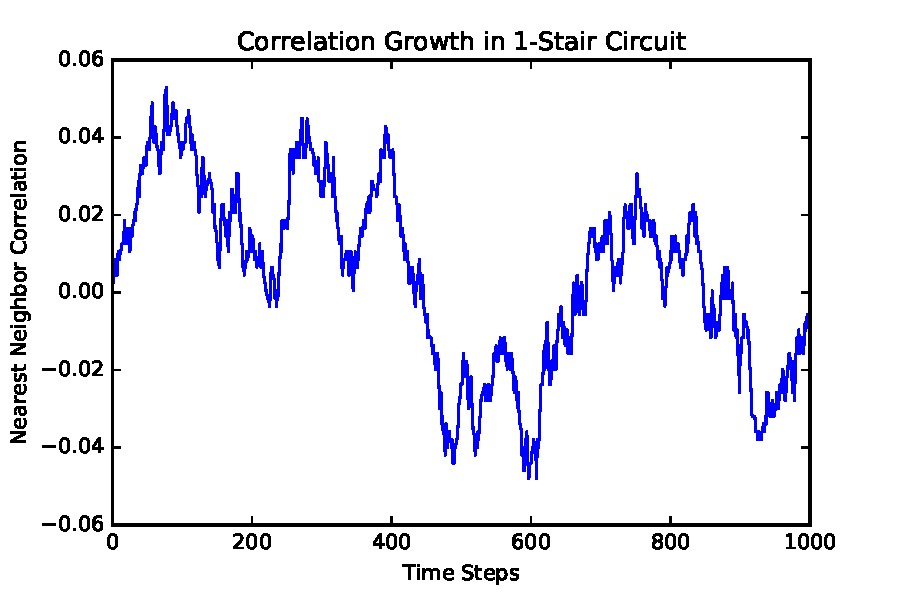
\includegraphics[width=.5\textwidth]{corrgrowth.pdf}
	\caption{\textbf{Correlation Growth for 0 slope.} Although the state starts out artificially anticorrelated, the correlation equilibrates after 400-600 time steps.}
	\label{fig:corrgrowth}
\end{figure}
The correlation saturates after 400-600 time steps, meaning the correlation of the initial state is not as important as the overall slope. For 1-stairs the correlation should asymptote to 0, as it appears to do. An interesting next step would be a way to analytically predict the correlation built by each circuit.